\textbf{Model podstawowy uczony na grafach czterowierzchołkowych}

Dokładność modelu podstawowego, uczonego na grafach z czterema wierzchołkami stopniowo rosnie,
zaczynając od około 40\% i osiągając prawie 90\% pod koniec procesu uczenia.
Może to sugoerować, że model dobrze uczy się na danych treningowych.
Dokładność na danych walidacyjnych jest zbliżona do wcześniej przytoczonej.
Wskazuje to, że model dobrze radzi sobie z generalizacją na nowych danych.

Strata na danych treningowych gwałtownie spada z około 1,75 do około 0,25 w ciągu pierwszych dziesięciu epok,
po czym stabilizuje się.
Wskazuje to na szybkie uczenie się na na danych treningowych.
Strata na danych walidacyjnych jest nieznacznie bardziej zmienna,
z kilkoma wzrostami w późniejszych epokach.
Może to sugerować trudności z generalizacją na nowych danych.

\begin{figure}[ht]
	\centering
	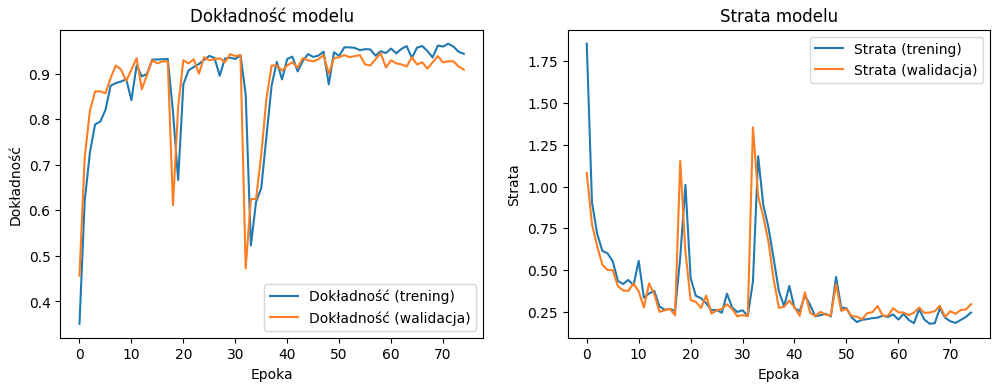
\includegraphics[height=5.5cm]{resources/tests/images/v3/base4_img.png}
	\caption{Wyniki testów dla modelu podstawowego, liczba wierzchołków = 4}
	\label{Fig:tests-base-1a}
\end{figure}
\FloatBarrier

Ogólnie rzecz biorąc, model wydaje się dobrze uczyć na danych treningowych i generalizować na danych walidacyjnych,
chociaż zmienność straty walidacyjnej może wskazywać na pewne problemy z przeuczeniem.

\begin{figure}[ht]
	\centering
	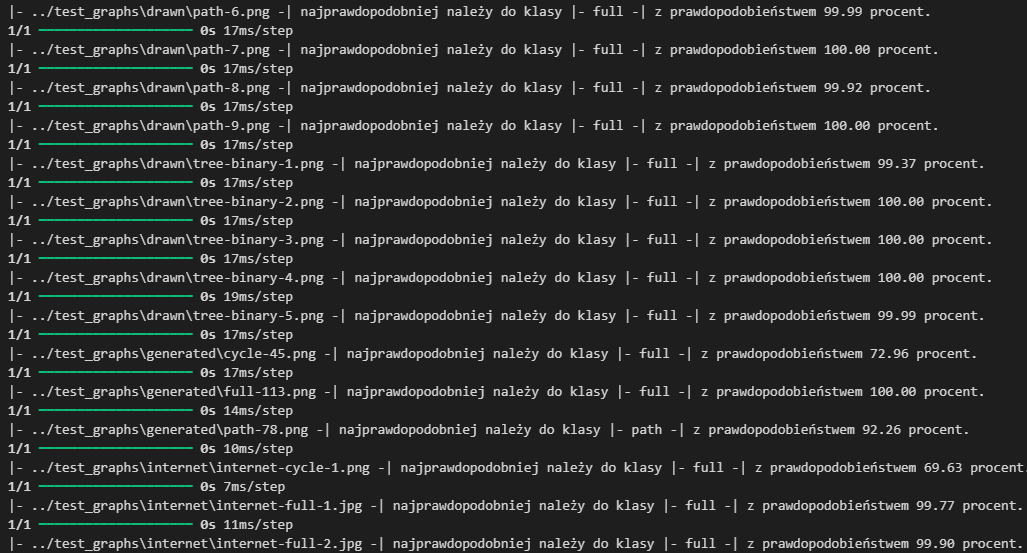
\includegraphics[width=14cm]{resources/tests/images/v3/base4_txt.png}
	\caption{Klasyfikacja obrazów zewnętrznych dla modelu podstawowego, liczba wierzchołków = 4}
	\label{Fig:tests-base-1b}
\end{figure}
\FloatBarrier

\begin{figure}[ht]
	\centering
	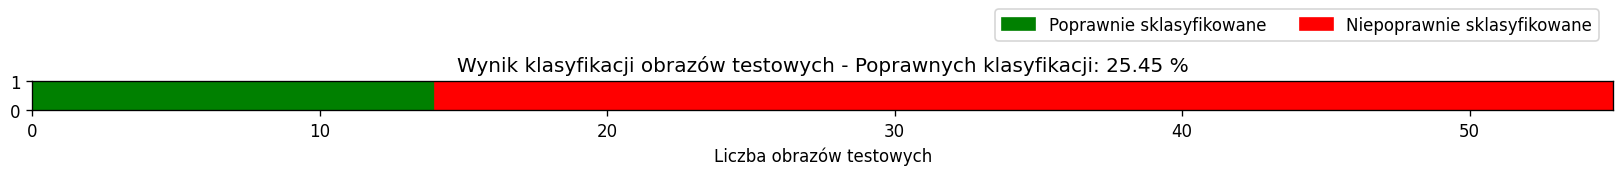
\includegraphics[width=14cm]{resources/tests/images/v3/base4_bar.png}
	\caption{Wizualizacja klasyfikacji obrazów zewnętrznych dla modelu podstawowego, liczba wierzchołków = 4}
	\label{Fig:tests-base-1c}
\end{figure}
\FloatBarrier

Model przewidział poprawnie 25\% grafów, co nie jest najgorszym wynikiem,
zaważając że jest to najbardziej podstawowa wersja testowanego modelu.

% \begin{figure}[ht]
% 	\centering
% 	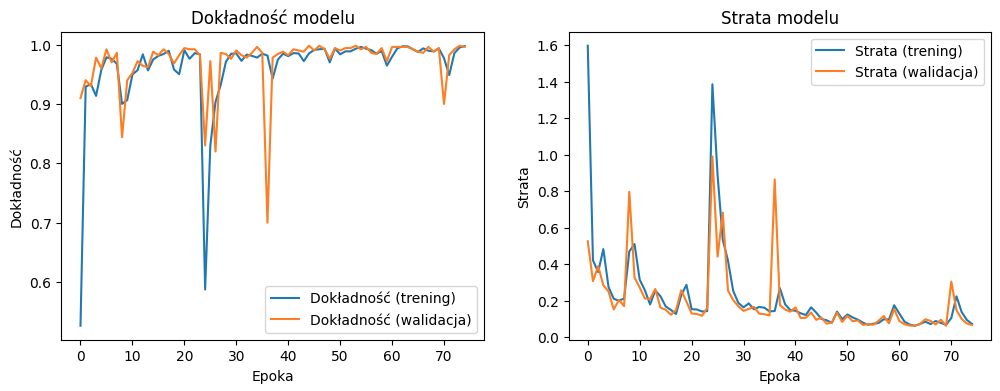
\includegraphics[height=5.5cm]{resources/tests/images/v3/base5_img.png}
% 	\caption{Wyniki testów dla modelu podstawowego, liczba wierzchołków = 5}
% 	\label{Fig:tests-base-2a}
% \end{figure}
% \FloatBarrier

% \begin{figure}[ht]
% 	\centering
% 	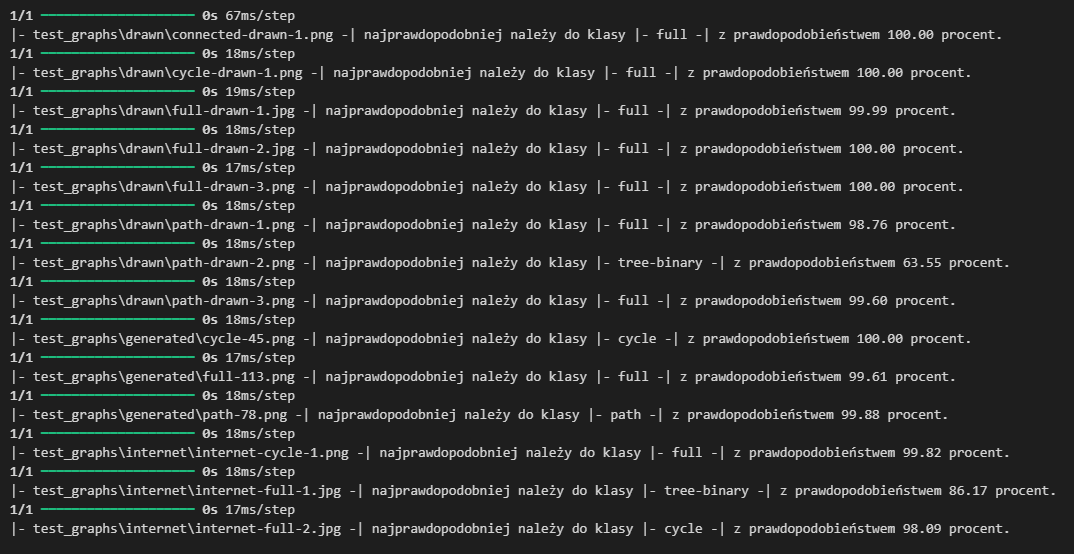
\includegraphics[width=14cm]{resources/tests/images/v3/base5_txt.png}
% 	\caption{Klasyfikacja obrazów zewnętrznych dla modelu podstawowego, liczba wierzchołków = 5}
% 	\label{Fig:tests-base-2b}
% \end{figure}
% \FloatBarrier

% \begin{figure}[ht]
% 	\centering
% 	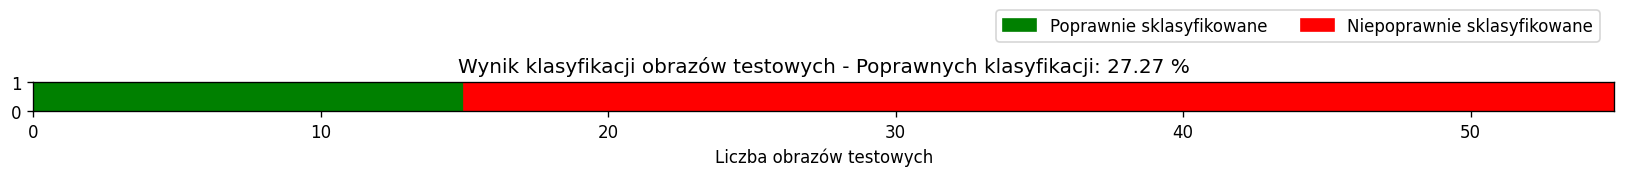
\includegraphics[width=14cm]{resources/tests/images/v3/base5_bar.png}
% 	\caption{Wizualizacja klasyfikacji obrazów zewnętrznych dla modelu podstawowego, liczba wierzchołków = 5}
% 	\label{Fig:tests-base-2c}
% \end{figure}
% \FloatBarrier

\textbf{Model podstawowy uczony na grafach sześciowierzchołkowych}

Kolejny warty uwagi wynik został uzyskany za pomocą podstaowego modelu, ale uczonego na grafach o sześciu wierzechołkach.
Dokładność zarówno dla zbioru treningowego, jak i walidacyjnego, bardzo szybko wzrasta już w kilku pierwszych epokach
i osiąga bardzo wysoki wynik, bo prawie 100\%.
Występuje kilka spadków obu krzywych, z czego jeden nawet do 80\%.
Ogólnie, po około 10 epokach, dokładność dla obu zestawów danych jest bardzo zbliżona i stabilizuje się na poziomie około 99\%.

Strata, podobnie jak dokładnośc, spada w ciągu początkowych epok procesu nauczania do niskich wartości, bo około 0,25.
W ciągu kolejnych epok, aż do końca, widać minimalny trend malejący, z trzema wzrostami straty do około wartości 0,5 na zbiorze walidacyjnym.
Może to oznaczać, że w tych punktach model napotyka na trudniejsze przypadki testowe.

\begin{figure}[ht]
	\centering
	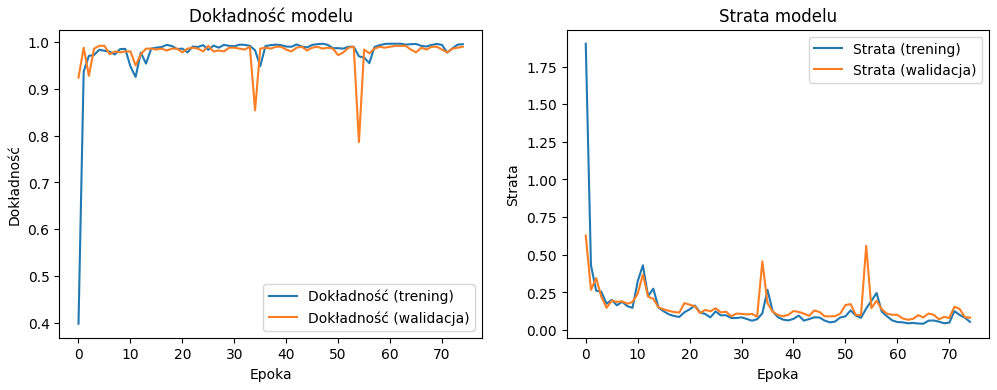
\includegraphics[height=5.5cm]{resources/tests/images/v3/base6_img.png}
	\caption{Wyniki testów dla modelu podstawowego, liczba wierzchołków = 6}
	\label{Fig:tests-base-3a}
\end{figure}
\FloatBarrier

Różnice między wartościami straty i dokładności dla zbioru walidacyjnego i testowego są niewielkie.
Nie widać również znaczących fluktuacji.
Krzywe dokładności i straty sugerują, że model może być poprawnie nauczony ogólnych wzorców
i nie być nadmiernie dopasowanym do danych treningowych.

\begin{figure}[ht]
	\centering
	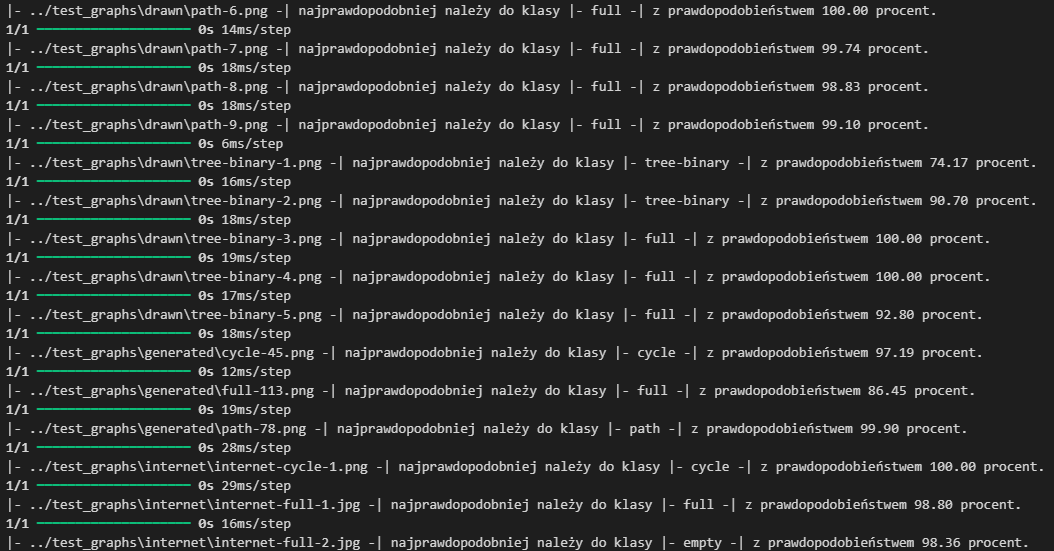
\includegraphics[width=14cm]{resources/tests/images/v3/base6_txt.png}
	\caption{Klasyfikacja obrazów zewnętrznych dla modelu podstawowego, liczba wierzchołków = 6}
	\label{Fig:tests-base-3b}
\end{figure}
\FloatBarrier

\begin{figure}[ht]
	\centering
	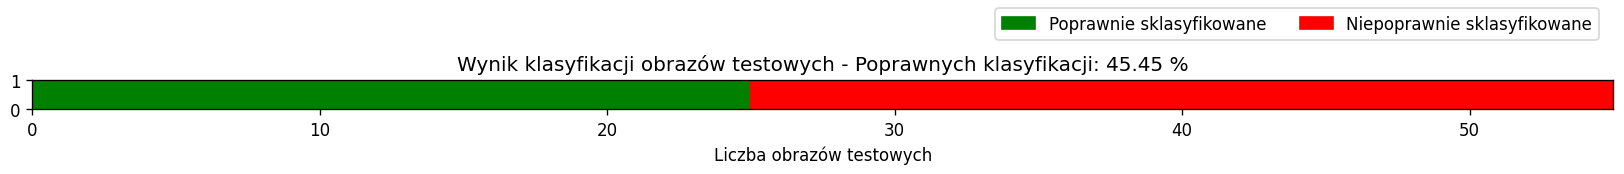
\includegraphics[width=14cm]{resources/tests/images/v3/base6_bar.png}
	\caption{Wizualizacja klasyfikacji obrazów zewnętrznych dla modelu podstawowego, liczba wierzchołków = 6}
	\label{Fig:tests-base-3c}
\end{figure}
\FloatBarrier

Model poprawnie klasyfikuje ponad 45\% przypadków grafów zewnętrznych, co jest zaskakująco wysokim wynikiem,
zważając na niską złożoność owego modelu.

% \begin{figure}[ht]
% 	\centering
% 	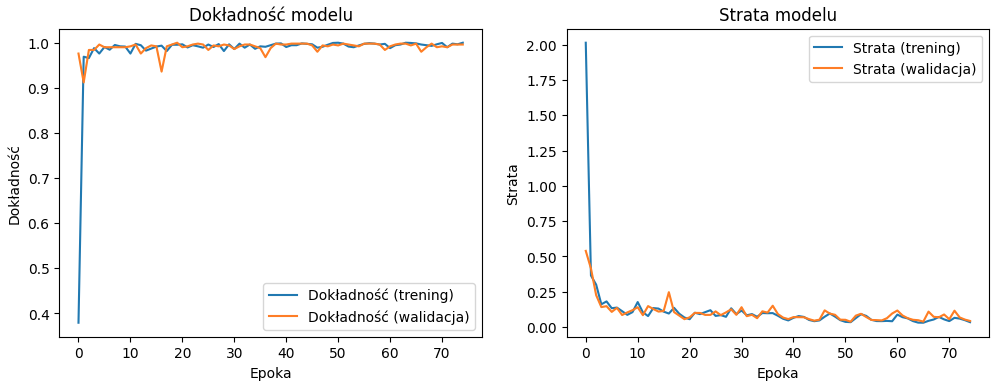
\includegraphics[height=5.5cm]{resources/tests/images/v3/base7_img.png}
% 	\caption{Wyniki testów dla modelu podstawowego, liczba wierzchołków = 7}
% 	\label{Fig:tests-base-4a}
% \end{figure}
% \FloatBarrier

% \begin{figure}[ht]
% 	\centering
% 	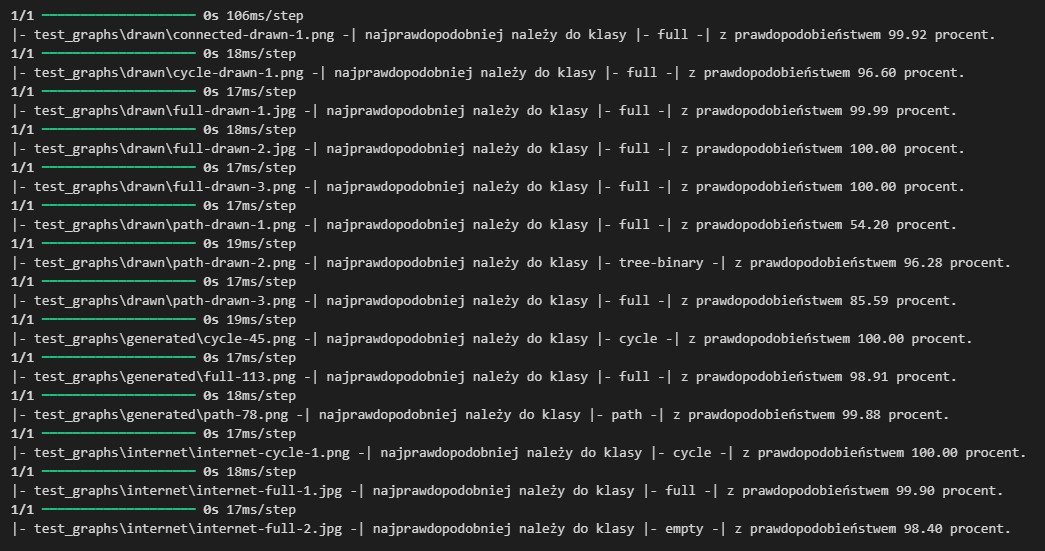
\includegraphics[width=14cm]{resources/tests/images/v3/base7_txt.png}
% 	\caption{Klasyfikacja obrazów zewnętrznych dla modelu podstawowego, liczba wierzchołków = 7}
% 	\label{Fig:tests-base-4b}
% \end{figure}
% \FloatBarrier

% \begin{figure}[ht]
% 	\centering
% 	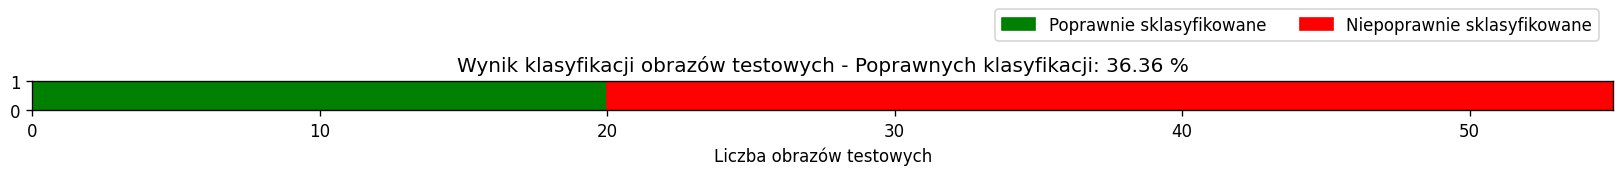
\includegraphics[width=14cm]{resources/tests/images/v3/base7_bar.png}
% 	\caption{Wizualizacja klasyfikacji obrazów zewnętrznych dla modelu podstawowego, liczba wierzchołków = 7}
% 	\label{Fig:tests-base-4c}
% \end{figure}
% \FloatBarrier